\section{Технический проект}
\subsection{Общая характеристика организации решения задачи}

Необходимо спроектировать и разработать базу данных для корпоративного мессенджера, которая должна обеспечивать надежное хранение и быстрый доступ к сообщениям, пользовательским данным и информации о группах.

База данных представляет собой структурированный набор взаимосвязанных таблиц, содержащих текстовую информацию (сообщения, имена пользователей), метаданные (временные отметки, идентификаторы) и системные данные (роли, статусы). База располагается в файле data.db и использует SQLite в качестве системы управления.

\subsection{Обоснование выбора технологии проектирования}

Для реализации корпоративного мессенджера рассмотрены различные СУБД, включая PostgreSQL, MySQL и SQLite. Выбор SQLite обусловлен следующими факторами:

\subsubsection{Система управления базами данных SQLite}

SQLite — встраиваемая реляционная СУБД, не требующая отдельного серверного процесса. Основные преимущества в контексте проекта:

\begin{itemize}
	\item Нулевая конфигурация — не требует администрирования
	\item Компактность — вся база в одном файле
	\item Высокая производительность для операций чтения/записи
	\item Полная поддержка транзакций ACID
\end{itemize}

\subsubsection{Достоинства SQLite для данного проекта}
\begin{itemize}
	\item Идеально подходит для приложений с одним пользователем или небольших рабочих групп
	\item Не требует отдельного сервера БД, что упрощает развертывание
	\item Поддерживает большинство возможностей SQL-92
\end{itemize}

\subsubsection{Ограничения SQLite}
\begin{itemize}
	\item Ограниченная поддержка одновременных записей (write-ahead logging включен)
	\item Максимальный размер базы данных около 140 TB (достаточно для корпоративного мессенджера)
	\item Отсутствие встроенной системы аутентификации пользователей
\end{itemize}

\subsection{Диаграмма компонентов базы данных}

Диаграмма компонентов базы данных представляет собой визуализацию структуры и взаимосвязей основных модулей системы хранения данных.

\begin{figure}[H]
\center{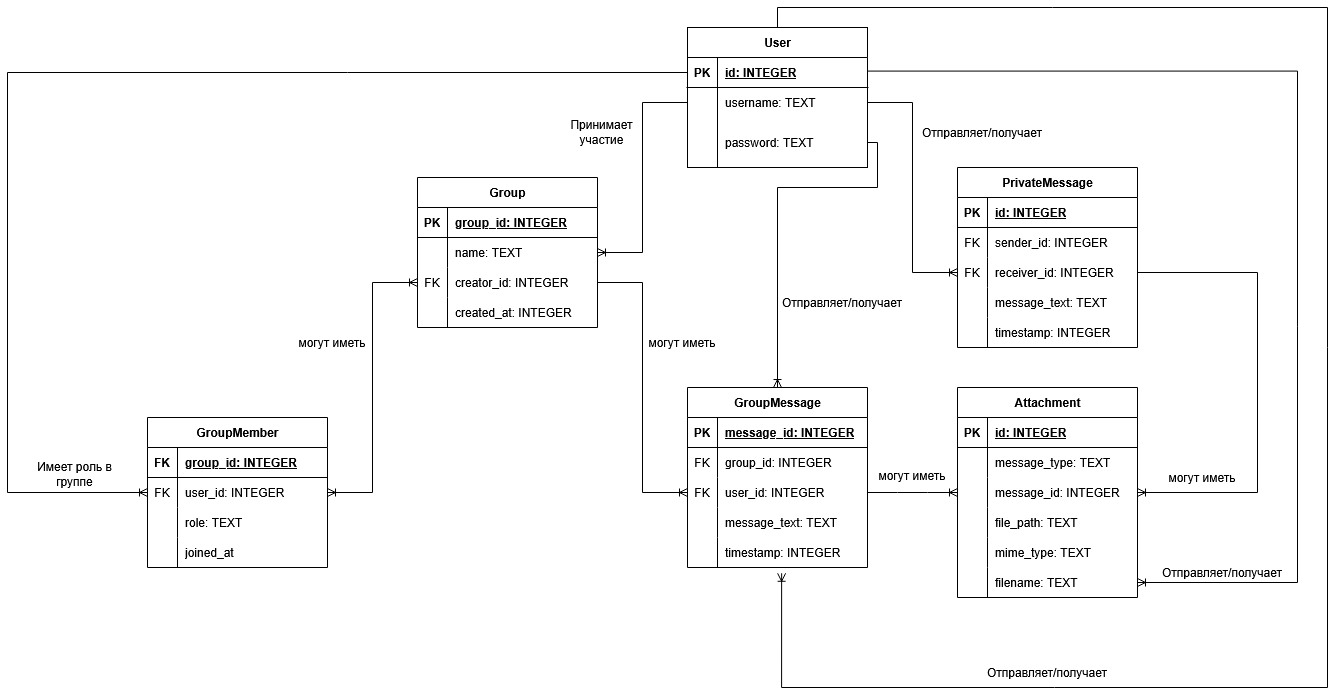
\includegraphics[width=1\linewidth]{ЕР модель}}
\caption{Диаграмма компонентов базы данных}
\label{comp:image}
\end{figure}

Диаграмма отражает логическую организацию таблиц, их назначение и ключевые взаимосвязи между ними.

\subsection{Таблицы базы данных}
\subsubsection{User - Пользователи системы}
\begin{xltabular}{\textwidth}{|l|l|X|}
	\caption{Атрибуты сущности "Пользователи"\label{user:table}}\\ \hline
	\centrow Поле & \centrow Тип & \centrow Описание \\ \hline
	\thead{id} & \thead{INTEGER} & Первичный ключ (PK), уникальный идентификатор пользователя \\ \hline
	\thead{username} & \thead{TEXT} & Имя пользователя (уникальное) \\ \hline
	\thead{password} & \thead{TEXT} & Хэшированный пароль пользователя \\ \hline
\end{xltabular}

Таблица "User" хранит информацию о зарегистрированных пользователях мессенджера. Каждый пользователь имеет уникальный идентификатор, имя пользователя и пароль. Является центральной сущностью системы, с которой связаны все остальные таблицы.

\subsubsection{Group - Групповые чаты}
\begin{xltabular}{\textwidth}{|l|l|X|}
	\caption{Атрибуты сущности "Групповые чаты"\label{group:table}}\\ \hline
	\centrow Поле & \centrow Тип & \centrow Описание \\ \hline
	\thead{group\_id} & \thead{INTEGER} & Первичный ключ (PK), ID группы \\ \hline
	\thead{name} & \thead{TEXT} & Название группы \\ \hline
	\thead{creator\_id} & \thead{INTEGER} & Внешний ключ (FK→User), ID создателя группы \\ \hline
	\thead{created\_at} & \thead{INTEGER} & Timestamp создания группы \\ \hline
\end{xltabular}

Таблица "Group" содержит информацию о групповых чатах. Каждая группа имеет уникальный идентификатор, название, создателя и время создания. Создатель группы автоматически становится владельцем (owner).

\subsubsection{GroupMember - Участники групп с ролями}
\begin{xltabular}{\textwidth}{|l|l|X|}
	\caption{Атрибуты сущности "Участники групп"\label{groupmember:table}}\\ \hline
	\centrow Поле & \centrow Тип & \centrow Описание \\ \hline
	\thead{group\_id} & \thead{INTEGER} & Внешний ключ (FK→Group), ID группы \\ \hline
	\thead{user\_id} & \thead{INTEGER} & Внешний ключ (FK→User), ID пользователя \\ \hline
	\thead{role} & \thead{TEXT} & Роль в группе: 'owner' (владелец), 'admin' (администратор), 'member' (участник) \\ \hline
	\thead{joined\_at} & \thead{INTEGER} & Timestamp вступления пользователя в группу \\ \hline
\end{xltabular}

Таблица "GroupMember" определяет состав участников групп и их роли. Реализует систему прав доступа, аналогичную Telegram, где владелец имеет максимальные права, администраторы - ограниченные права управления, а участники - базовые права.

\subsubsection{GroupMessage - Сообщения в группах}
\begin{xltabular}{\textwidth}{|l|l|X|}
	\caption{Атрибуты сущности "Групповые сообщения"\label{groupmessage:table}}\\ \hline
	\centrow Поле & \centrow Тип & \centrow Описание \\ \hline
	\thead{message\_id} & \thead{INTEGER} & Первичный ключ (PK), ID сообщения \\ \hline
	\thead{group\_id} & \thead{INTEGER} & Внешний ключ (FK→Group), ID группы \\ \hline
	\thead{user\_id} & \thead{INTEGER} & Внешний ключ (FK→User), ID отправителя \\ \hline
	\thead{message\_text} & \thead{TEXT} & Текст сообщения (может быть пустым для сообщений с вложениями) \\ \hline
	\thead{timestamp} & \thead{INTEGER} & Время отправки сообщения (timestamp) \\ \hline
\end{xltabular}

Таблица "GroupMessage" хранит все сообщения, отправленные в групповых чатах. Каждое сообщение связано с группой и пользователем-отправителем. Поддерживает текстовые сообщения и сообщения с вложениями (через таблицу Attachment).

На рисунке \ref{data:image} представлена схема обмена данными между сценариями компонента при вызове компонента на странице сайта.

\begin{figure}[H]
\center{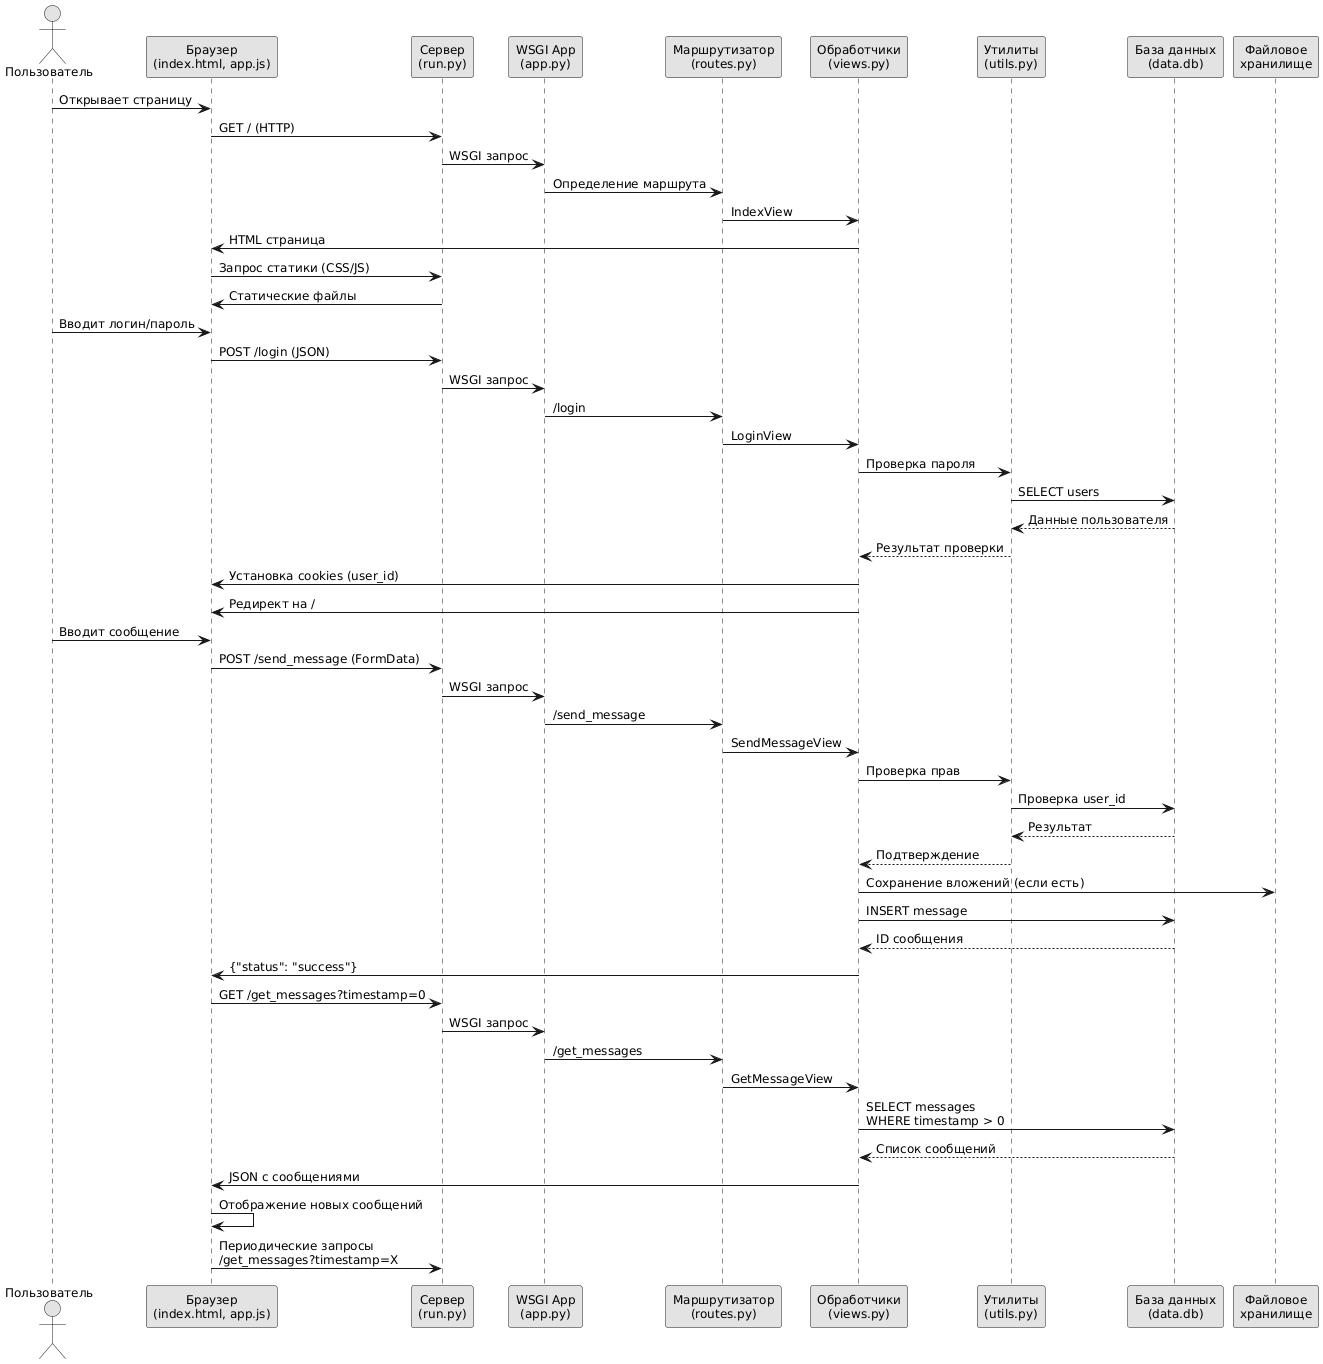
\includegraphics[width=1\linewidth]{Диаграмма последовательности}}
\caption{Диаграмма компонентов}
\label{data:image}
\end{figure}

\subsection{Описание диаграммы последовательности работы корпоративного мессенджера}

\begin{enumerate}[leftmargin=*,label=\textbf{\arabic*.}]
	\item \textbf{Загрузка страницы (инициализация)}
	\begin{itemize}
		\item Пользователь открывает в браузере главную страницу (\texttt{index.html})
		\item Браузер отправляет HTTP GET-запрос на сервер
		\item Серверный скрипт \texttt{run.py} (Waitress) получает запрос
		\item Запрос передаётся в WSGI-приложение (\texttt{app.py})
		\item Маршрутизатор (\texttt{routes.py}) определяет обработчик \texttt{IndexView}
		\item Пользователю возвращается HTML-страница и статические файлы (CSS/JS)
	\end{itemize}
	
	\item \textbf{Процесс аутентификации}
	\begin{itemize}
		\item Пользователь вводит логин и пароль в форму входа
		\item Браузер отправляет POST /login запрос (JSON)
		\item \texttt{LoginView} проверяет учётные данные:
		\begin{itemize}
			\item Через \texttt{utils.py} выполняется SQL-запрос к таблице \texttt{users}
			\item Пароль проверяется с помощью bcrypt
		\end{itemize}
		\item При успешной аутентификации:
		\begin{itemize}
			\item Устанавливается cookie с \texttt{user\_id}
			\item Происходит редирект на главную страницу
		\end{itemize}
	\end{itemize}
	
	\item \textbf{Отправка нового сообщения}
	\begin{itemize}
		\item Пользователь вводит текст и/или прикрепляет файлы
		\item Браузер формирует FormData и отправляет POST /send\_message
		\item \texttt{SendMessageView} выполняет:
		\begin{itemize}
			\item Проверку прав через cookies
			\item Сохранение файлов в \texttt{static/uploads}
			\item Запись сообщения в БД (таблицы \texttt{messages} или \texttt{group\_messages})
		\end{itemize}
		\item Клиент получает JSON с результатом операции
	\end{itemize}
	
	\item \textbf{Получение сообщений (реализация чата)}
	\begin{itemize}
		\item Браузер периодически опрашивает сервер (GET /get\_messages)
		\item \texttt{GetMessageView} запрашивает новые сообщения из БД
		\item Сервер возвращает JSON с массивом сообщений
		\item Браузер динамически обновляет интерфейс чата
	\end{itemize}
	
	\item \textbf{Особенности работы}
	\begin{itemize}
		\item Все запросы проходят через единую точку входа (\texttt{app.py})
		\item Маршрутизатор выбирает соответствующий View-класс
		\item Бизнес-логика сосредоточена в \texttt{views.py}
		\item Работа с БД вынесена в \texttt{utils.py}
		\item Файлы хранятся локально в файловой системе
		\item Состояние сессии поддерживается через cookies
	\end{itemize}
\end{enumerate}

\subsection{Диаграмма размещения}

Диаграмма размещения (рис.~\ref{place:image}) отражает физические взаимосвязи между программными и аппаратными компонентами системы.

\begin{figure}[ht]
\center{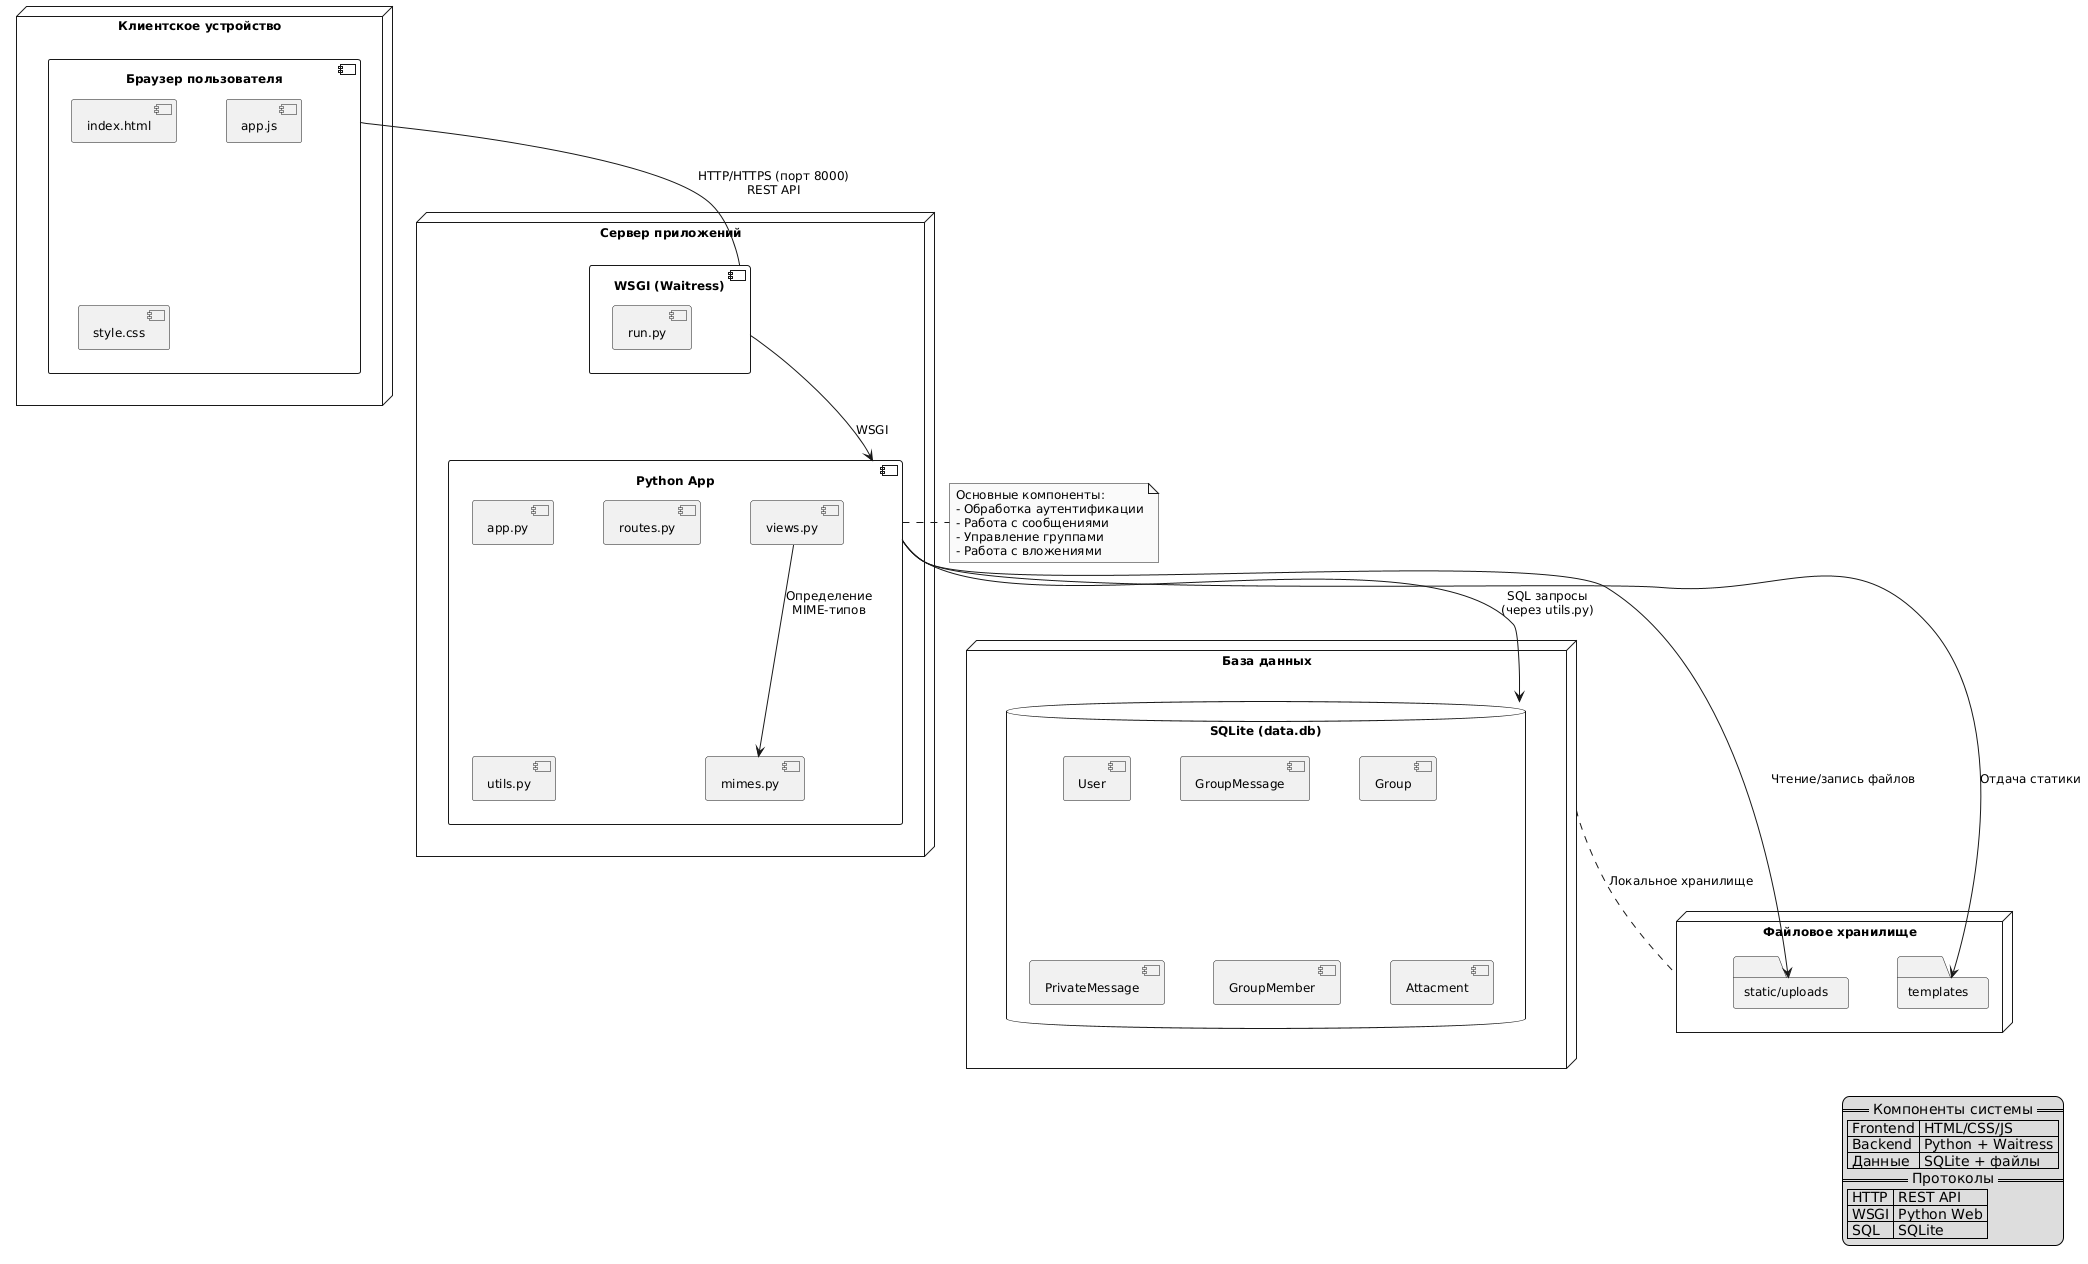
\includegraphics[width=1\linewidth]{Диаграмма развёртывания}}
\caption{Диаграмма развёртывания}
\label{place:image}
\end{figure}

Она является хорошим средством для показа маршрутов перемещения объектов и компонентов в распределенной системе.

